\tikzset{every picture/.style={line width=0.75pt}} %set default line width to 0.75pt        

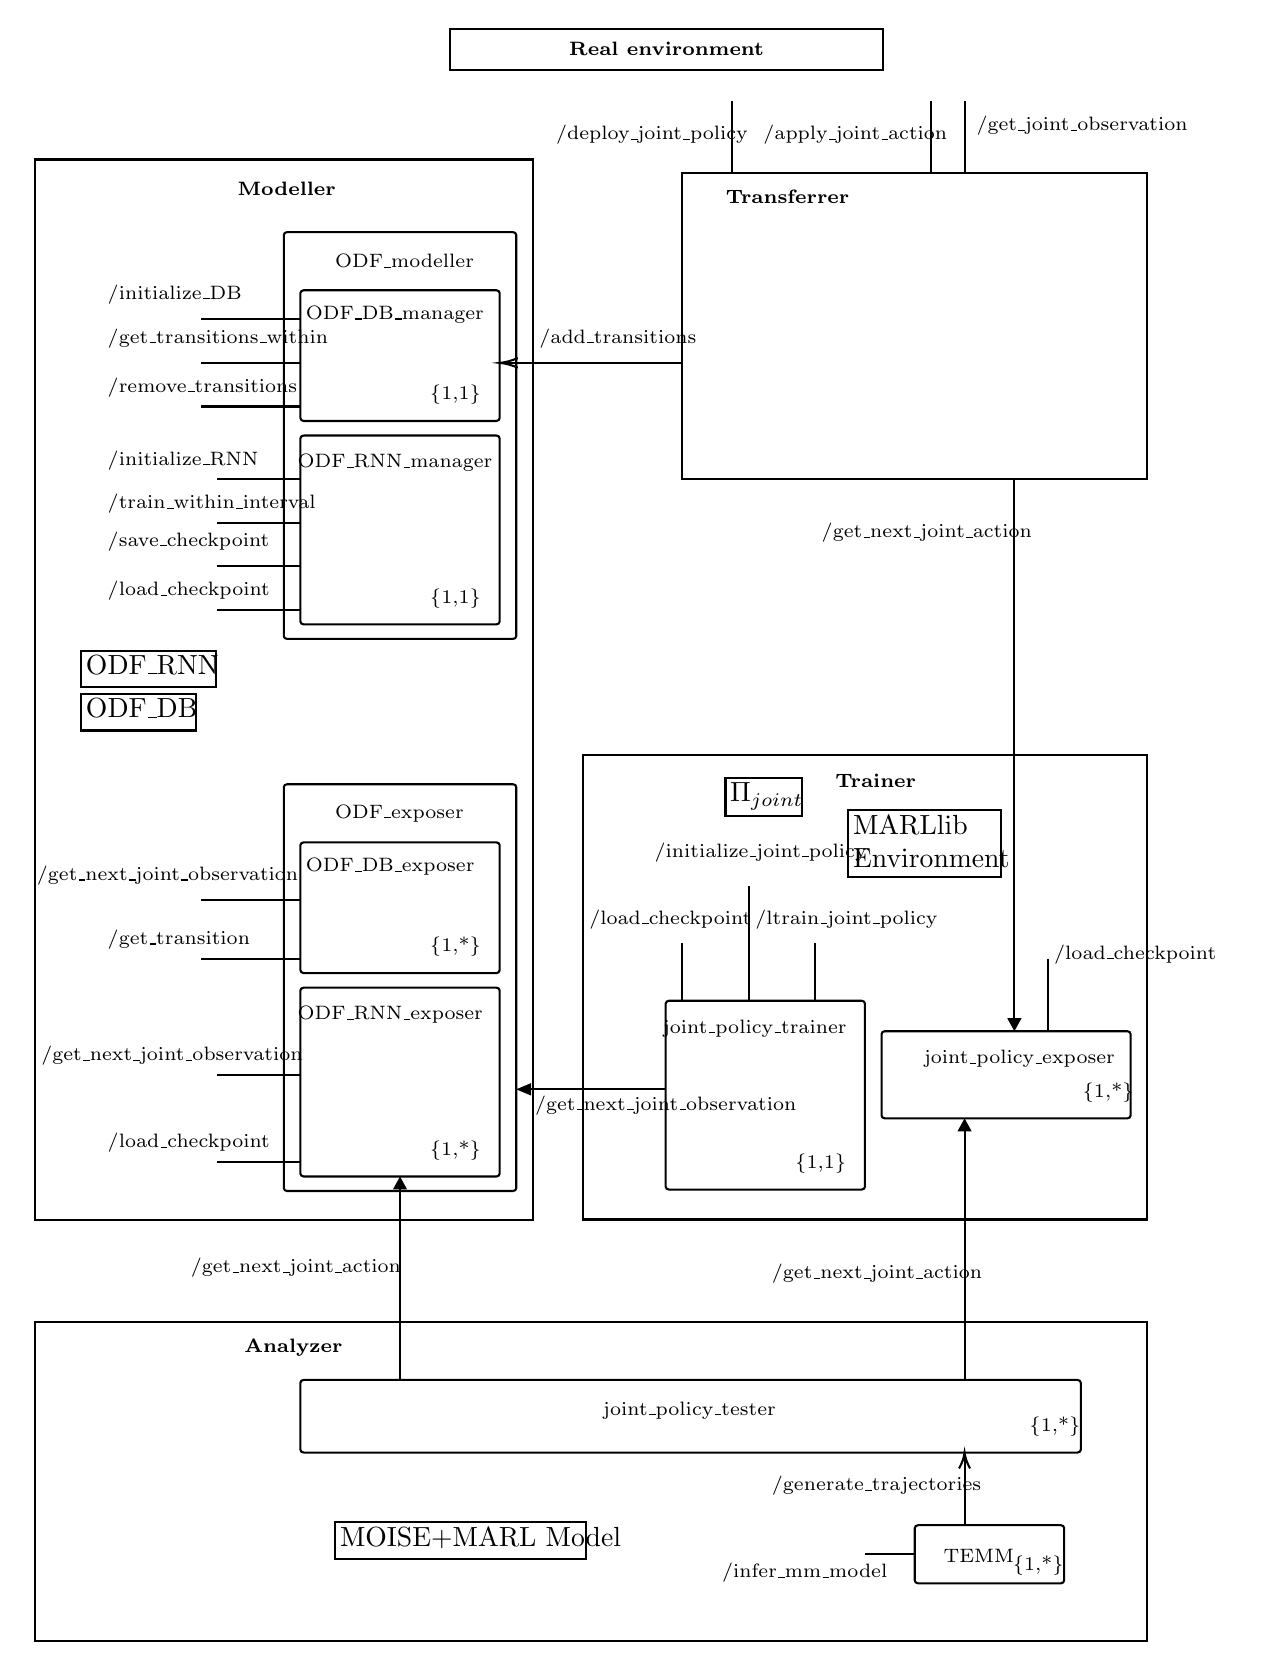
\begin{tikzpicture}[x=0.75pt,y=0.75pt,yscale=-0.7,xscale=0.8]
%uncomment if require: \path (0,2390); %set diagram left start at 0, and has height of 2390

%Shape: Rectangle [id:dp14572306266206714] 
\draw   (10,270) -- (310,270) -- (310,1000) -- (10,1000) -- cycle ;
%Shape: Rectangle [id:dp3731534134783796] 
\draw   (400,279.56) -- (680,279.56) -- (680,490) -- (400,490) -- cycle ;
%Shape: Rectangle [id:dp6847392398744736] 
\draw   (340,680) -- (680,680) -- (680,999.6) -- (340,999.6) -- cycle ;
%Shape: Rectangle [id:dp4686800871113095] 
\draw   (260,180) -- (521.12,180) -- (521.12,208.18) -- (260,208.18) -- cycle ;
%Straight Lines [id:da4123404851401349] 
\draw    (430,280) -- (430,230) ;
%Straight Lines [id:da3928144550795716] 
\draw    (550,280) -- (550,230) ;
%Straight Lines [id:da30255118033461437] 
\draw    (570,230) -- (570,280) ;
%Straight Lines [id:da5888988670167654] 
\draw    (170.01,380) -- (110.01,380) ;
%Straight Lines [id:da6443924304465367] 
\draw    (170.01,440) -- (110.01,440) ;
%Straight Lines [id:da9943122625114935] 
\draw    (170.01,490) -- (120.01,490) ;
%Straight Lines [id:da6811218206422291] 
\draw    (170.01,520) -- (120.01,520) ;
%Straight Lines [id:da8718454315815845] 
\draw    (170.01,550) -- (120.01,550) ;
%Straight Lines [id:da9210291628916512] 
\draw    (170.01,580) -- (120.01,580) ;
%Shape: Rectangle [id:dp7085799582359258] 
\draw   (160.01,322) .. controls (160.01,320.9) and (160.91,320) .. (162.01,320) -- (298.01,320) .. controls (299.12,320) and (300.01,320.9) .. (300.01,322) -- (300.01,598) .. controls (300.01,599.1) and (299.12,600) .. (298.01,600) -- (162.01,600) .. controls (160.91,600) and (160.01,599.1) .. (160.01,598) -- cycle ;
%Shape: Rectangle [id:dp652788159293541] 
\draw   (170.01,462) .. controls (170.01,460.9) and (170.91,460) .. (172.01,460) -- (288.01,460) .. controls (289.12,460) and (290.01,460.9) .. (290.01,462) -- (290.01,588) .. controls (290.01,589.1) and (289.12,590) .. (288.01,590) -- (172.01,590) .. controls (170.91,590) and (170.01,589.1) .. (170.01,588) -- cycle ;
%Shape: Rectangle [id:dp25963751229564913] 
\draw   (170.01,362) .. controls (170.01,360.9) and (170.91,360) .. (172.01,360) -- (288.01,360) .. controls (289.12,360) and (290.01,360.9) .. (290.01,362) -- (290.01,448) .. controls (290.01,449.1) and (289.12,450) .. (288.01,450) -- (172.01,450) .. controls (170.91,450) and (170.01,449.1) .. (170.01,448) -- cycle ;
%Straight Lines [id:da6040204166418095] 
\draw    (170.01,780) -- (110.01,780) ;
%Straight Lines [id:da9471295078437141] 
\draw    (170.01,820) -- (110.01,820) ;
%Straight Lines [id:da3685224310052644] 
\draw    (170.01,900) -- (120.01,900) ;
%Straight Lines [id:da905328785948986] 
\draw    (170.01,960) -- (120.01,960) ;
%Shape: Rectangle [id:dp526681929477721] 
\draw   (160.01,702) .. controls (160.01,700.9) and (160.91,700) .. (162.01,700) -- (298.01,700) .. controls (299.12,700) and (300.01,700.9) .. (300.01,702) -- (300.01,978) .. controls (300.01,979.1) and (299.12,980) .. (298.01,980) -- (162.01,980) .. controls (160.91,980) and (160.01,979.1) .. (160.01,978) -- cycle ;
%Shape: Rectangle [id:dp2733198576306253] 
\draw   (170.01,842) .. controls (170.01,840.9) and (170.91,840) .. (172.01,840) -- (288.01,840) .. controls (289.12,840) and (290.01,840.9) .. (290.01,842) -- (290.01,968) .. controls (290.01,969.1) and (289.12,970) .. (288.01,970) -- (172.01,970) .. controls (170.91,970) and (170.01,969.1) .. (170.01,968) -- cycle ;
%Shape: Rectangle [id:dp5529320606155974] 
\draw   (170.01,742) .. controls (170.01,740.9) and (170.91,740) .. (172.01,740) -- (288.01,740) .. controls (289.12,740) and (290.01,740.9) .. (290.01,742) -- (290.01,828) .. controls (290.01,829.1) and (289.12,830) .. (288.01,830) -- (172.01,830) .. controls (170.91,830) and (170.01,829.1) .. (170.01,828) -- cycle ;
%Straight Lines [id:da7760382959944025] 
\draw    (400,410) -- (292.01,410) ;
\draw [shift={(290.01,410)}, rotate = 360] [color={rgb, 255:red, 0; green, 0; blue, 0 }  ][line width=0.75]    (10.93,-3.29) .. controls (6.95,-1.4) and (3.31,-0.3) .. (0,0) .. controls (3.31,0.3) and (6.95,1.4) .. (10.93,3.29)   ;
%Shape: Rectangle [id:dp2721892662967862] 
\draw   (390,851.01) .. controls (390,849.9) and (390.9,849.01) .. (392,849.01) -- (508,849.01) .. controls (509.1,849.01) and (510,849.9) .. (510,851.01) -- (510,977.01) .. controls (510,978.11) and (509.1,979.01) .. (508,979.01) -- (392,979.01) .. controls (390.9,979.01) and (390,978.11) .. (390,977.01) -- cycle ;
%Shape: Rectangle [id:dp8918015245746698] 
\draw   (520,872) .. controls (520,870.9) and (520.9,870) .. (522,870) -- (668,870) .. controls (669.1,870) and (670,870.9) .. (670,872) -- (670,928) .. controls (670,929.1) and (669.1,930) .. (668,930) -- (522,930) .. controls (520.9,930) and (520,929.1) .. (520,928) -- cycle ;
%Straight Lines [id:da3289618444790672] 
\draw    (400,849.01) -- (400,809.01) ;
%Straight Lines [id:da6293406567564059] 
\draw    (230,973) -- (230,1110) ;
\draw [shift={(230,970)}, rotate = 90] [fill={rgb, 255:red, 0; green, 0; blue, 0 }  ][line width=0.08]  [draw opacity=0] (8.93,-4.29) -- (0,0) -- (8.93,4.29) -- cycle    ;
%Straight Lines [id:da17135272871940388] 
\draw    (620,820) -- (620,870) ;
%Shape: Rectangle [id:dp9907074530473785] 
\draw   (10,1070.4) -- (680,1070.4) -- (680,1290) -- (10,1290) -- cycle ;
%Straight Lines [id:da23202835635421737] 
\draw    (600,867) -- (600,490) ;
\draw [shift={(600,870)}, rotate = 270] [fill={rgb, 255:red, 0; green, 0; blue, 0 }  ][line width=0.08]  [draw opacity=0] (8.93,-4.29) -- (0,0) -- (8.93,4.29) -- cycle    ;
%Shape: Rectangle [id:dp6818448791531506] 
\draw   (170,1112) .. controls (170,1110.9) and (170.9,1110) .. (172,1110) -- (638,1110) .. controls (639.1,1110) and (640,1110.9) .. (640,1112) -- (640,1158) .. controls (640,1159.1) and (639.1,1160) .. (638,1160) -- (172,1160) .. controls (170.9,1160) and (170,1159.1) .. (170,1158) -- cycle ;
%Straight Lines [id:da2641055390549132] 
\draw    (303,910) -- (390,910) ;
\draw [shift={(300,910)}, rotate = 0] [fill={rgb, 255:red, 0; green, 0; blue, 0 }  ][line width=0.08]  [draw opacity=0] (8.93,-4.29) -- (0,0) -- (8.93,4.29) -- cycle    ;
%Straight Lines [id:da3485570792881172] 
\draw    (440,849.01) -- (440,770) ;
%Straight Lines [id:da1204785129243755] 
\draw    (480,849.01) -- (480,809.01) ;
%Straight Lines [id:da2707272780297001] 
\draw    (570,933) -- (570,1110) ;
\draw [shift={(570,930)}, rotate = 90] [fill={rgb, 255:red, 0; green, 0; blue, 0 }  ][line width=0.08]  [draw opacity=0] (8.93,-4.29) -- (0,0) -- (8.93,4.29) -- cycle    ;
%Shape: Rectangle [id:dp1171149343188016] 
\draw   (540,1212) .. controls (540,1210.9) and (540.9,1210) .. (542,1210) -- (628,1210) .. controls (629.1,1210) and (630,1210.9) .. (630,1212) -- (630,1248) .. controls (630,1249.1) and (629.1,1250) .. (628,1250) -- (542,1250) .. controls (540.9,1250) and (540,1249.1) .. (540,1248) -- cycle ;
%Straight Lines [id:da714391461732099] 
\draw    (570,1210) -- (570,1162) ;
\draw [shift={(570,1160)}, rotate = 90] [color={rgb, 255:red, 0; green, 0; blue, 0 }  ][line width=0.75]    (10.93,-3.29) .. controls (6.95,-1.4) and (3.31,-0.3) .. (0,0) .. controls (3.31,0.3) and (6.95,1.4) .. (10.93,3.29)   ;
%Straight Lines [id:da4258377282431203] 
\draw    (540,1230) -- (510,1230) ;
%Straight Lines [id:da40346082889425894] 
\draw    (170,410) -- (110,410) ;


% Text Node
\draw (105,393) node  [font=\scriptsize] [align=left] {\begin{minipage}[lt]{61.23pt}\setlength\topsep{0pt}
/get\_transitions\_within
\end{minipage}};
% Text Node
\draw (608.5,1238) node  [font=\scriptsize] [align=left] {\begin{minipage}[lt]{11.33pt}\setlength\topsep{0pt}
\{1,*\}
\end{minipage}};
% Text Node
\draw (618.5,1142) node  [font=\scriptsize] [align=left] {\begin{minipage}[lt]{11.33pt}\setlength\topsep{0pt}
\{1,*\}
\end{minipage}};
% Text Node
\draw    (191,1208) -- (342,1208) -- (342,1233) -- (191,1233) -- cycle  ;
\draw (192,1209) node [anchor=north west][inner sep=0.75pt]   [align=left] {MOISE+MARL Model};
% Text Node
\draw (475,1243) node  [font=\scriptsize] [align=left] {\begin{minipage}[lt]{61.23pt}\setlength\topsep{0pt}
/infer\_mm\_model
\end{minipage}};
% Text Node
\draw (505,1183) node  [font=\scriptsize] [align=left] {\begin{minipage}[lt]{61.23pt}\setlength\topsep{0pt}
/generate\_trajectories
\end{minipage}};
% Text Node
\draw (580,1231) node  [font=\scriptsize] [align=left] {\begin{minipage}[lt]{27.2pt}\setlength\topsep{0pt}
TEMM
\end{minipage}};
% Text Node
\draw (505,1037) node  [font=\scriptsize] [align=left] {\begin{minipage}[lt]{61.23pt}\setlength\topsep{0pt}
/get\_next\_joint\_action
\end{minipage}};
% Text Node
\draw (535,527) node  [font=\scriptsize] [align=left] {\begin{minipage}[lt]{61.23pt}\setlength\topsep{0pt}
/get\_next\_joint\_action
\end{minipage}};
% Text Node
\draw (384.99,920.91) node  [font=\scriptsize] [align=left] {\begin{minipage}[lt]{88.42pt}\setlength\topsep{0pt}
/get\_next\_joint\_observation
\end{minipage}};
% Text Node
\draw (417,1131) node  [font=\scriptsize] [align=left] {\begin{minipage}[lt]{77.52pt}\setlength\topsep{0pt}
joint\_policy\_tester
\end{minipage}};
% Text Node
\draw (167,1087.5) node  [font=\scriptsize] [align=left] {\begin{minipage}[lt]{36.96pt}\setlength\topsep{0pt}
\textbf{Analyzer}
\end{minipage}};
% Text Node
\draw    (500,718) -- (592,718) -- (592,764) -- (500,764) -- cycle  ;
\draw (501,719) node [anchor=north west][inner sep=0.75pt]   [align=left] {MARLlib\\Environment};
% Text Node
\draw (650.56,912) node  [font=\scriptsize] [align=left] {\begin{minipage}[lt]{11.33pt}\setlength\topsep{0pt}
\{1,*\}
\end{minipage}};
% Text Node
\draw (485,961.01) node  [font=\scriptsize] [align=left] {\begin{minipage}[lt]{20.4pt}\setlength\topsep{0pt}
\{1,1\}
\end{minipage}};
% Text Node
\draw (675,817) node  [font=\scriptsize] [align=left] {\begin{minipage}[lt]{61.23pt}\setlength\topsep{0pt}
/load\_checkpoint
\end{minipage}};
% Text Node
\draw (495,793) node  [font=\scriptsize] [align=left] {\begin{minipage}[lt]{61.21pt}\setlength\topsep{0pt}
/ltrain\_joint\_policy
\end{minipage}};
% Text Node
\draw    (426,696) -- (472,696) -- (472,722) -- (426,722) -- cycle  ;
\draw (427,697) node [anchor=north west][inner sep=0.75pt]   [align=left] {$\displaystyle \Pi _{joint}$};
% Text Node
\draw (155,1033) node  [font=\scriptsize] [align=left] {\begin{minipage}[lt]{61.23pt}\setlength\topsep{0pt}
/get\_next\_joint\_action
\end{minipage}};
% Text Node
\draw (440,747) node  [font=\scriptsize] [align=left] {\begin{minipage}[lt]{68.01pt}\setlength\topsep{0pt}
/initialize\_joint\_policy
\end{minipage}};
% Text Node
\draw (395,793) node  [font=\scriptsize] [align=left] {\begin{minipage}[lt]{61.23pt}\setlength\topsep{0pt}
/load\_checkpoint
\end{minipage}};
% Text Node
\draw (581.5,889) node  [font=\scriptsize] [align=left] {\begin{minipage}[lt]{43.07pt}\setlength\topsep{0pt}
joint\_policy\_exposer
\end{minipage}};
% Text Node
\draw (453,868.01) node  [font=\scriptsize] [align=left] {\begin{minipage}[lt]{77.52pt}\setlength\topsep{0pt}
joint\_policy\_trainer
\end{minipage}};
% Text Node
\draw (365,393) node  [font=\scriptsize] [align=left] {\begin{minipage}[lt]{61.23pt}\setlength\topsep{0pt}
/add\_transitions
\end{minipage}};
% Text Node
\draw (265,952) node  [font=\scriptsize] [align=left] {\begin{minipage}[lt]{20.4pt}\setlength\topsep{0pt}
\{1,*\}
\end{minipage}};
% Text Node
\draw (265.01,812) node  [font=\scriptsize] [align=left] {\begin{minipage}[lt]{20.4pt}\setlength\topsep{0pt}
\{1,*\}
\end{minipage}};
% Text Node
\draw (265.01,572) node  [font=\scriptsize] [align=left] {\begin{minipage}[lt]{20.4pt}\setlength\topsep{0pt}
\{1,1\}
\end{minipage}};
% Text Node
\draw (265.01,432) node  [font=\scriptsize] [align=left] {\begin{minipage}[lt]{20.4pt}\setlength\topsep{0pt}
\{1,1\}
\end{minipage}};
% Text Node
\draw (105.01,947) node  [font=\scriptsize] [align=left] {\begin{minipage}[lt]{61.23pt}\setlength\topsep{0pt}
/load\_checkpoint
\end{minipage}};
% Text Node
\draw (65.01,887) node  [font=\scriptsize] [align=left] {\begin{minipage}[lt]{61.23pt}\setlength\topsep{0pt}
/get\_next\_joint\_observation
\end{minipage}};
% Text Node
\draw (105.01,807) node  [font=\scriptsize] [align=left] {\begin{minipage}[lt]{61.23pt}\setlength\topsep{0pt}
/get\_transition
\end{minipage}};
% Text Node
\draw (85,763) node  [font=\scriptsize] [align=left] {\begin{minipage}[lt]{88.42pt}\setlength\topsep{0pt}
/get\_next\_joint\_observation
\end{minipage}};
% Text Node
\draw (233.01,859) node  [font=\scriptsize] [align=left] {\begin{minipage}[lt]{77.52pt}\setlength\topsep{0pt}
ODF\_RNN\_exposer
\end{minipage}};
% Text Node
\draw (230.01,756.92) node  [font=\scriptsize] [align=left] {\begin{minipage}[lt]{68pt}\setlength\topsep{0pt}
ODF\_DB\_exposer
\end{minipage}};
% Text Node
\draw (233.01,720) node  [font=\scriptsize] [align=left] {\begin{minipage}[lt]{50.44pt}\setlength\topsep{0pt}
ODF\_exposer
\end{minipage}};
% Text Node
\draw (105.01,567) node  [font=\scriptsize] [align=left] {\begin{minipage}[lt]{61.23pt}\setlength\topsep{0pt}
/load\_checkpoint
\end{minipage}};
% Text Node
\draw (105.01,533) node  [font=\scriptsize] [align=left] {\begin{minipage}[lt]{61.23pt}\setlength\topsep{0pt}
/save\_checkpoint
\end{minipage}};
% Text Node
\draw (105.01,507) node  [font=\scriptsize] [align=left] {\begin{minipage}[lt]{61.23pt}\setlength\topsep{0pt}
/train\_within\_interval
\end{minipage}};
% Text Node
\draw (105.01,477) node  [font=\scriptsize] [align=left] {\begin{minipage}[lt]{61.23pt}\setlength\topsep{0pt}
/initialize\_RNN
\end{minipage}};
% Text Node
\draw (105.01,427) node  [font=\scriptsize] [align=left] {\begin{minipage}[lt]{61.23pt}\setlength\topsep{0pt}
/remove\_transitions
\end{minipage}};
% Text Node
\draw (105.01,363) node  [font=\scriptsize] [align=left] {\begin{minipage}[lt]{61.23pt}\setlength\topsep{0pt}
/initialize\_DB
\end{minipage}};
% Text Node
\draw (233.01,479) node  [font=\scriptsize] [align=left] {\begin{minipage}[lt]{77.52pt}\setlength\topsep{0pt}
ODF\_RNN\_manager
\end{minipage}};
% Text Node
\draw (230.01,376.92) node  [font=\scriptsize] [align=left] {\begin{minipage}[lt]{68pt}\setlength\topsep{0pt}
ODF\_DB\_manager
\end{minipage}};
% Text Node
\draw (233.01,340) node  [font=\scriptsize] [align=left] {\begin{minipage}[lt]{50.44pt}\setlength\topsep{0pt}
ODF\_modeller
\end{minipage}};
% Text Node
\draw    (38.01,638) -- (107.01,638) -- (107.01,663) -- (38.01,663) -- cycle  ;
\draw (39.01,639) node [anchor=north west][inner sep=0.75pt]   [align=left] {ODF\_DB};
% Text Node
\draw    (38.01,608) -- (119.01,608) -- (119.01,633) -- (38.01,633) -- cycle  ;
\draw (39.01,609) node [anchor=north west][inner sep=0.75pt]   [align=left] {ODF\_RNN};
% Text Node
\draw (375,253) node  [font=\scriptsize] [align=left] {\begin{minipage}[lt]{61.23pt}\setlength\topsep{0pt}
/deploy\_joint\_policy
\end{minipage}};
% Text Node
\draw (626.5,247) node  [font=\scriptsize] [align=left] {\begin{minipage}[lt]{59.13pt}\setlength\topsep{0pt}
/get\_joint\_observation
\end{minipage}};
% Text Node
\draw (492,253) node  [font=\scriptsize] [align=left] {\begin{minipage}[lt]{51.74pt}\setlength\topsep{0pt}
/apply\_joint\_action
\end{minipage}};
% Text Node
\draw (390.56,194.09) node  [font=\scriptsize] [align=left] {\begin{minipage}[lt]{73.9pt}\setlength\topsep{0pt}
\begin{center}
\textbf{Real environment}
\end{center}

\end{minipage}};
% Text Node
\draw (523,697.5) node  [font=\scriptsize] [align=left] {\begin{minipage}[lt]{36.96pt}\setlength\topsep{0pt}
\textbf{Trainer}
\end{minipage}};
% Text Node
\draw (457,293) node  [font=\scriptsize] [align=left] {\begin{minipage}[lt]{36.96pt}\setlength\topsep{0pt}
\begin{center}
\textbf{Transferrer}
\end{center}

\end{minipage}};
% Text Node
\draw (163,290) node  [font=\scriptsize] [align=left] {\begin{minipage}[lt]{36.96pt}\setlength\topsep{0pt}
\textbf{Modeller}
\end{minipage}};


\end{tikzpicture}